%% 
%% Copyright 2007-2020 Elsevier Ltd
%% 
%% This file is part of the 'Elsarticle Bundle'.
%% ---------------------------------------------
%% 
%% It may be distributed under the conditions of the LaTeX Project Public
%% License, either version 1.2 of this license or (at your option) any
%% later version.  The latest version of this license is in
%%    http://www.latex-project.org/lppl.txt
%% and version 1.2 or later is part of all distributions of LaTeX
%% version 1999/12/01 or later.
%% 
%% The list of all files belonging to the 'Elsarticle Bundle' is
%% given in the file `manifest.txt'.
%% 

%% Template article for Elsevier's document class `elsarticle'
%% with numbered style bibliographic references
%% SP 2008/03/01
%%
%% 
%%
%% $Id: elsarticle-template-num.tex 190 2020-11-23 11:12:32Z rishi $
%%
%%
\documentclass[preprint,12pt]{elsarticle}

%% Use the option review to obtain double line spacing
%% \documentclass[authoryear,preprint,review,12pt]{elsarticle}

%% Use the options 1p,twocolumn; 3p; 3p,twocolumn; 5p; or 5p,twocolumn
%% for a journal layout:
%% \documentclass[final,1p,times]{elsarticle}
%% \documentclass[final,1p,times,twocolumn]{elsarticle}
%% \documentclass[final,3p,times]{elsarticle}
%% \documentclass[final,3p,times,twocolumn]{elsarticle}
%% \documentclass[final,5p,times]{elsarticle}
%% \documentclass[final,5p,times,twocolumn]{elsarticle}

%% For including figures, graphicx.sty has been loaded in
%% elsarticle.cls. If you prefer to use the old commands
%% please give \usepackage{epsfig}

%% The amssymb package provides various useful mathematical symbols
\usepackage{amssymb}
\usepackage{amsmath}
\usepackage{graphicx}
\usepackage[font={small,it}]{caption}
\usepackage{subcaption}
\graphicspath{{figures/}}
%% The amsthm package provides extended theorem environments
%% \usepackage{amsthm}

%% The lineno packages adds line numbers. Start line numbering with
%% \begin{linenumbers}, end it with \end{linenumbers}. Or switch it on
%% for the whole article with \linenumbers.
%% \usepackage{lineno}

\journal{Computer Methods in Applied Mechanics and Engineering          }

\begin{document}
%.......................................................................
%  Define some latex commands to reduce the length of the equations
%......................................................................
\newcommand{\pd}[2]{\ensuremath{\frac{\partial#1}{\partial#2}}  }
\newcommand{\pbox}[1]{\ensuremath{\parbox[b]{.27\linewidth}{ \scriptsize \textsf {#1}}}  }
\newcommand{\pboxsmall}[1]{\ensuremath{\parbox[c]{.2\linewidth}{\scriptsize{#1}}}  }
\newcommand{\graybox}[1]{\psboxit{box .7 setgray fill}{\fbox{#1}} }
\newcommand{\half}          {\ensuremath{\tiny{\frac{1}{2}}}}
%
%.......................................................................
%  SINGLE MATEERIAL
%......................................................................
%..............................
%  no time superscript
%..............................                
\newcommand{\U}             {{\vec{U}}}                    
\newcommand{\uo}            {\ensuremath{\vec{U}_o}}                  
\newcommand{\delt}          {\ensuremath{\Delta{t}} }                 
\newcommand{\delx}          {\ensuremath{\Delta{x}} }                 
\newcommand{\dely}          {\ensuremath{\Delta{y}} }                 
\newcommand{\delz}          {\ensuremath{\Delta{z}} }
\newcommand{\delV}          {\ensuremath{\Delta{V}} }                 
\newcommand{\rhoo}          {\ensuremath{\rho_o}}
\newcommand{\rr}            {\ensuremath{\mathbf{r}}   }                     
\newcommand{\sumarea}       {\ensuremath{\sum_{i=1}^{n}}} 
\newcommand{\XCC}           {\ensuremath{\frac{\delx}{2}}}
\newcommand{\YCC}           {\ensuremath{\frac{\dely}{2}}}
\newcommand{\ZCC}           {\ensuremath{\frac{\delz}{2}}}
\newcommand{\angler}        {\ensuremath{\langle\mathbf{r}\rangle}   }        
%
%..............................
%  time n quantities
%..............................
\newcommand{\un}            {\ensuremath{\vec{U}^{n}}}
\newcommand{\unc}           {\ensuremath{\vec{U}^{n^{c}}}}               
\newcommand{\Tnc}           {\ensuremath{T^{n^{c}}}}                     
\newcommand{\pnc}           {\ensuremath{p^{n^c}} }                      
\newcommand{\en}            {\ensuremath{e^{n}}}                         
\newcommand{\mnc}           {\ensuremath{m^{n^{c}}}}                     
\newcommand{\Vnf}           {\ensuremath{V^{n^{f}}}} 
\newcommand{\Vn}            {\ensuremath{V^{n}} }                    
\newcommand{\mnf}           {\ensuremath{m^{n^{f}}}}                
\newcommand{\unf}           {\ensuremath{\vec{U}^{n^{f}}}}          
\newcommand{\rhonf}         {\ensuremath{\rho^{n^{f}}}}             
\newcommand{\rhonc}         {\ensuremath{\rho^{n^{c}}}}             
\newcommand{\rhoncl}        {\ensuremath{\rho^{n^{c}}_r}}           
\newcommand{\spvol}         {\ensuremath{ \upsilon^{n^{c}} } }
\newcommand{\uvelnc}        {\ensuremath{ u^{n^{c}} } }
\newcommand{\vvelnc}        {\ensuremath{ v^{n^{c}} } }
\newcommand{\wvelnc}        {\ensuremath{ w^{n^{c}} } }
\newcommand{\momnc}         {\ensuremath{(m\vec{U})^{n^{c}} } }
\newcommand{\engnc}         {\ensuremath{E^{n^{c}} } }
%..............................
%  n quantities I,J,K
%..............................
\newcommand{\unIJK}         {\ensuremath{u^{n}_{i,j,k}}}
\newcommand{\TnIJK}         {\ensuremath{T^{n}_{i,j,k}}}
\newcommand{\cvIJK}         {\ensuremath{c_{v_{i,j,k}}}}
\newcommand{\uncIJK}        {\ensuremath{u^{n^{c}}_{i,j,k}}}
\newcommand{\vnIJK}         {\ensuremath{v^{n}_{i,j,k}}}
\newcommand{\VnIJK}         {\ensuremath{V^{n}_{i,j,k}}}
\newcommand{\vncIJK}        {\ensuremath{v^{n^{c}}_{i,j,k}}}
\newcommand{\wnIJK}         {\ensuremath{w^{n}_{i,j,k}}}
\newcommand{\wncIJK}        {\ensuremath{w^{n^{c}}_{i,j,k}}}
\newcommand{\uijkl}         {\ensuremath{ u^{*^{f}}_{{i,j,k,L}}}}
\newcommand{\uijkr}         {\ensuremath{ u^{*^{f}}_{{i,j,k,R}}}}
\newcommand{\vijkt}         {\ensuremath{ v^{*^{f}}_{{i,j,k,T}}}}
\newcommand{\vijkb}         {\ensuremath{ v^{*^{f}}_{{i,j,k,B}}}}
\newcommand{\wijkf}         {\ensuremath{ w^{*^{f}}_{{i,j,k,FR}}}}
\newcommand{\wijkbk}        {\ensuremath{ w^{*^{f}}_{{i,j,k,BK}}}}
\newcommand{\rhonIJK}       {\ensuremath{\rho^{n}_{i,j,k}}}
%
%..............................
%  n + 1 quantities
%..............................
\newcommand{\nadv}          {\text{\tiny{n+1}}}                             
\newcommand{\unnL}          {\ensuremath{\vec{U}^{\nadv^{L}}}}              
\newcommand{\unnf}          {\ensuremath{\vec{U}^{\nadv^{{f}}}}}          
\newcommand{\unnc}          {\ensuremath{\vec{U}^{\nadv^{c}}}}      
\newcommand{\VnnL}          {\ensuremath{V^{\nadv^{L}}}}
\newcommand{\uvelstar}      {\ensuremath{ u^{\nadv^{*^{f}}}}  }             
\newcommand{\vvelstar}      {\ensuremath{ v^{\nadv^{*^{f}}}}  }             
\newcommand{\wvelstar}      {\ensuremath{ w^{\nadv^{*^{f}}}}  }             
\newcommand{\TnnL}          {\ensuremath{ T^{\nadv^{L}}}  }
\newcommand{\Tnnc}          {\ensuremath{ T^{\nadv^{c}}}  }
\newcommand{\ustar}         {\ensuremath{\vec{U}^{\nadv^{*^{f}}}}}          
\newcommand{\udummy}        {\ensuremath{\hat{ \vec{U} }^{\nadv^{f}}  } }   
\newcommand{\pstar}         {\ensuremath{p^{\nadv^{*^{f}}}}}                
\newcommand{\pnnLc}         {\ensuremath{p^{\nadv^{L^c}}} }                 
\newcommand{\rhonnc}        {\ensuremath{\rho^{\nadv{^{c}}}}}
\newcommand{\rhonnL}        {\ensuremath{\rho^{\nadv{^{L}}}}} 
\newcommand{\rhonnf}        {\ensuremath{\rho^{\nadv{^{f}}}}}          
\newcommand{\delpc}         {\ensuremath{ \Delta p^{\nadv^{c}}  } }         
\newcommand{\momnnL}        {\ensuremath{(m\vec{U})^{\nadv^{L}} } }
\newcommand{\momnnc}        {\ensuremath{(m\vec{U})^{\nadv^{c}} } }
\newcommand{\massnnc}       {\ensuremath{m^{\nadv^{c}} } }
\newcommand{\massnnL}       {\ensuremath{m^{\nadv^{L}} } }
\newcommand{\massnnLf}      {\ensuremath{m^{\nadv^{L}^{f}} } }
\newcommand{\engnnc}        {\ensuremath{E^{\nadv^{c}} } }
\newcommand{\engnnL}        {\ensuremath{e^{\nadv^{L}} } }
\newcommand{\volfracnn}     {\ensuremath{\theta^{\nadv} } }
\newcommand{\delmomnn}      {\ensuremath{\Delta(m\vec{U})^{\nadv} } }  
\newcommand{\delengnn}      {\ensuremath{\Delta(mT)^{\nadv} } } 
\newcommand{\delmassnn}     {\ensuremath{\Delta(m)^{\nadv} } }
%          
%..............................
%  n + 1 quantities, i,j 
%..............................
\newcommand{\VnnLIJK}       {\ensuremath{V^{\nadv^{L}}_{i,j,k}}}
\newcommand{\unnLIJK}       {\ensuremath{u^{\nadv^{L}}_{i,j,k}}}
\newcommand{\vnnLIJK}       {\ensuremath{v^{\nadv^{L}}_{i,j,k}}}
\newcommand{\wnnLIJK}       {\ensuremath{w^{\nadv^{L}}_{i,j,k}}}
\newcommand{\rhonnLIJK}     {\ensuremath{\rho^{\nadv^{L}}_{i,j,k}}}
\newcommand{\massnnLIJK}     {\ensuremath{m^{\nadv^{L}}_{i,j,k}}}
\newcommand{\ennLIJK}     {\ensuremath{e^{\nadv^{L}}_{i,j,k}}}

\newcommand{\unnFIJK}       {\ensuremath{u^{\nadv^{*^{f}}}_{i,j,k}}}
\newcommand{\vnnFIJK}       {\ensuremath{v^{\nadv^{*^{f}}}_{i,j,k}}}
\newcommand{\wnnFIJK}       {\ensuremath{w^{\nadv^{*^{f}}}_{i,j,k}}}

%
%......................................................................
%  MULTIMATEERIAL
%......................................................................
\newcommand{\um}            {\ensuremath{\vec{U}_{m}}}                  
\newcommand{\rhom}          {\ensuremath{\rho_m}}                       
%
%..............................
%  n quantities
%..............................
\newcommand{\Vnm}           {\ensuremath{V^{n}_{m}}}                    
\newcommand{\massnm}        {\ensuremath{m^{n}_{m}}}                    
\newcommand{\unm}           {\ensuremath{\vec{U}^{n}_{m}}}
\newcommand{\unLm}          {\ensuremath{\vec{U}^{n^{L}}_{m}}}              
\newcommand{\Tnm}           {\ensuremath{T^{n}_{m}}}
\newcommand{\TnLm}          {\ensuremath{T^{n^{L}}_{m}}}                    
\newcommand{\engnm}         {\ensuremath{e^{n}_{m}}} 
\newcommand{\rhonm}         {\ensuremath{\rho^{n}_{m}}}
\newcommand{\momnm}         {\ensuremath{(m\vec{U})^{n}_{m} } }
%                   
%..............................
%  n+1 quantities 
%..............................
\newcommand{\unnm}          {\ensuremath{ \vec{U}^{\nadv}_{m}}  }
\newcommand{\unnLm}         {\ensuremath{\vec{U}^{\nadv^{L}}_{m}}}
\newcommand{\Tnnm}          {\ensuremath{ T^{\nadv}_{m}}  }
\newcommand{\TnnLm}         {\ensuremath{T^{\nadv^{L}}_{m}}}
\newcommand{\alpham}        {\ensuremath{\alpha_m}}                     
\newcommand{\VnnLm}         {\ensuremath{V^{\nadv^{L}}_{m}}}            
\newcommand{\rhonnLm}       {\ensuremath{\rho^{\nadv^{L}}_{m}}}
\newcommand{\ustarm}        {\ensuremath{\vec{U}^{\nadv^{*^{f}}}_{m}}}
\newcommand{\momnnm}        {\ensuremath{(m\vec{U})^{\nadv}_{m} } }
\newcommand{\momnnLm}       {\ensuremath{(m\vec{U})^{\nadv^{L}}_{m} } }
\newcommand{\massnnm}       {\ensuremath{m^{\nadv}_{m} } }
\newcommand{\massnnLm}      {\ensuremath{m^{\nadv^{L}}_{m} } }
\newcommand{\engnnLm}       {\ensuremath{(m c_v T)^{\nadv^{L}}_m } }
\newcommand{\engnnm}        {\ensuremath{(m c_v T)^{\nadv}_m } }           
%

%
%  RESET THE COUNTERS
\setcounter{equation}{0}
\setcounter{figure}{0}
\setcounter{section}{0}
%

\begin{frontmatter}

%% Title, authors and addresses

%% use the tnoteref command within \title for footnotes;
%% use the tnotetext command for theassociated footnote;
%% use the fnref command within \author or \address for footnotes;
%% use the fntext command for theassociated footnote;
%% use the corref command within \author for corresponding author footnotes;
%% use the cortext command for theassociated footnote;
%% use the ead command for the email address,
%% and the form \ead[url] for the home page:
%% \title{Title\tnoteref{label1}}
%% \tnotetext[label1]{}
%% \author{Name\corref{cor1}\fnref{label2}}
%% \ead{email address}
%% \ead[url]{home page}
%% \fntext[label2]{}
%% \cortext[cor1]{}
%% \affiliation{organization={},
%%             addressline={},
%%             city={},
%%             postcode={},
%%             state={},
%%             country={}}
%% \fntext[label3]{}

\title{MPMICE2}

%% use optional labels to link authors explicitly to addresses:
%% \author[label1,label2]{}
%% \affiliation[label1]{organization={},
%%             addressline={},
%%             city={},
%%             postcode={},
%%             state={},
%%             country={}}
%%
%% \affiliation[label2]{organization={},
%%             addressline={},
%%             city={},
%%             postcode={},
%%             state={},
%%             country={}}

\author{Quoc Anh Tran}

\affiliation{organization={},%Department and Organization
            addressline={}, 
            city={},
            postcode={}, 
            state={},
            country={}}

\begin{abstract}
%% Text of abstract
Abtract here
\end{abstract}

%%Graphical abstract
\begin{graphicalabstract}
%\includegraphics{grabs}
\end{graphicalabstract}

%%Research highlights
\begin{highlights}
\item Research highlight 1
\item Research highlight 2
\end{highlights}

\begin{keyword}
%% keywords here, in the form: keyword \sep keyword

%% PACS codes here, in the form: \PACS code \sep code

%% MSC codes here, in the form: \MSC code \sep code
%% or \MSC[2008] code \sep code (2000 is the default)

\end{keyword}

\end{frontmatter}

%
%
%
%______________________________________________________________________
%   Table of Contents    
%______________________________________________________________________
\newpage
\setcounter{secnumdepth}{-2}
\tableofcontents
%% \linenumbers

%______________________________________________________________________
\newpage
%
%
\section{\textsf{Nomenclature}}
\begin{tabular}{lll}
\\
\pmb{General variables}\\
\underline{\textsf{Variable}} & \underline{\textsf{Dimensions}} & \underline{\textsf{Description} }\\
$V$      				&   $[L^3]$     & Representative volume\\
$n$      				&           	& Porosity\\
$\pmb{\sigma}$ 			&  $[M/L^2]$ 	& Total stress tensor\\
$\delt$       			&  $[t]$      	& Time increment\\
$\pmb{b}$ 			    &  $[L/t]$ 	    & Gravity acceleration\\
$c_v$                   &  $[L^2/t^2]$  & Constant volume specific heat\\
$f_{fs}$ 		  	    &  $[ML//t^2]$ 	& Drag forces in momentum exchange term\\
$f^{int}$ 		  	    &  $[ML//t^2]$ 	& Internal forces\\
$f^{ext}$ 		  	    &  $[ML//t^2]$ 	& External forces\\
$q_{fs}$ 		  	    &  $[ML//t^2]$ 	& Heat exchange term\\
$S$ 		  	    	&            	& Shape function\\
$\nabla S$ 				&            	& Gradient of shape function\\
\pmb{Solid phase}\\
\underline{\textsf{Variable}} & \underline{\textsf{Dimensions}} & \underline{\textsf{Description} }\\
$m_s   $       			&  $[M]$      	& Solid mass\\
$\rho_s$				&	$[M/L^3]$  	& Solid density\\
$\phi_s$				     &	$-]$  	& Solid volume fraction\\
$\overline{\rho}_s$		&	$[M/L^3]$  	& Average Solid density\\
$\pmb{x}_s$   			&  	$[L]$    	& Solid Position vector\\
$\pmb{U}_s$   			&  	$[L/t]$    	& Solid Velocity vector\\
$\pmb{U}_s$   			&  	$[L/t]$    	& Solid Velocity gradient vector\\
$\pmb{a}_s$   			&  	$[L/t^2]$   & Solid Acceleration vector\\
$\pmb{\sigma}^\prime$ 	&  $[M/L^2]$ 	& Effective Stress tensor\\
$e_s$         			&  $[L^2/t^2]$  & Solid Internal energy \\   
$T_s$           		&  $[T]$      	& Solid Temperature\\
$\pmb{F}_s$     		&       	    & Solid Deformation gradient\\
$V_s$     				&  $[L^3]$      & Volume\\
\end{tabular}

\newpage
%
%
\begin{tabular}{lll}
\\
\pmb{Fluid phase}\\
\underline{\textsf{Variable}} & \underline{\textsf{Dimensions}} & \underline{\textsf{Description} }\\
$m_f   $       			&  $[M]$      	& Fluid mass\\
$\rho_f$	    		            &   $[M/L^3]$  	& Fluid density\\
$\phi_f$				      &   $-]$  	& Fluid volume fraction\\
$\overline{\rho}_f$		&  $[M/L^3]$  	& Average Fluid density\\
$\pmb{U}_f$   			&  $[L/t]$    	& Fluid Velocity vector\\
$\pmb{\sigma}_f$ 		&  $[M/L^2]$ 	& Fluid stress tensor\\
$\Delta p_f$ 				&  $[M/L^2]$ 	& Fluid isotropic pressure\\
$\pmb{\tau}_f$ 			&  $[M/L^2]$ 	& Fluid shear stress tensor\\
$p_f$ 		  			&  $[M/L^2]$ 	& Isotropic pressure\\
$e_f$         			&  $[L^2/t^2]$  & Fluid Internal energy $(c_vT_f)$ of the material per unit mass \\   
$T_f$           		&  $[T]$      	& Fluid Temperature\\
$\upsilon_f$    		&  $[L^3/M]$  	& Fluid Specific volume $\frac{1}{\rho_f}$\\
$\alpha_f$    		    &  $[1/T]$  	& Thermal expansion\\
$\mu$    		    &  $[M/L^2 T]$  	& Fluid vicousity\\

\pmb{Superscript}\\
\underline{\textsf{Variable}} & \underline{\textsf{Dimensions}} & \underline{\textsf{Description} }\\
$n$           			&               &    Current time step\\
$L$           			&               &    Lagrangian values\\
$n+1$         			&               &    Next time step\\
\pmb{Subscript}\\
$c$           			&               &    Cell-centered quantity\\
$p$           			&               &    Particle quantity\\
$i$           			&               &    Node quantity\\
$FC$           			&             	&    Face-centered quantity\\
$L, R $       			&             	&    Left and Right cell faces\\
\end{tabular}
\newpage
%
%__________________________________________________
%% main text
\section{\textsf{Introduction}}
write introduction
%_______________________________
\section{\textsf{Theory and formulation}}

%_______________________________
\subsection{\textsf{Assumptions}}

%_______________________________
\subsection{\textsf{Governing equations}}

%_______________________________
\subsubsection{Balance equations}

%_______________________________
\subsubsection{Equation of state for fluid plases}

%
%
\begin{figure}
\center
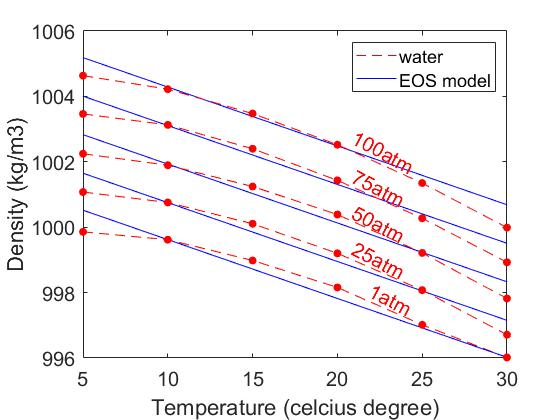
\includegraphics[scale=.5]{water1.jpg}
\caption{Equation of state of water}
\label{fig:water1}
\end{figure}
%
%

%_______________________________
\subsubsection{Constitutive soil model}

%_______________________________
\subsubsection{Momentum and Energy exchange model}

%_______________________________
\subsubsection{Turbulent model}

%_______________________________
\section{\textsf{Numerical implementation}}

%_______________________________
\section{\textsf{Numerical examples}}
All input files and the analytical calculations in this section are provided in the Github repository \footnote{https://github.com/QuocAnh90/Uintah NTNU} for the reproduction of the numerical results.\\
%_______________________________
\subsection{\textsf{Fluid Flow through isothermal porous media}}
Fluid flow through porous media is important in many engineering disciplines, like predicting water flow in soil. Fluid flow velocity in one dimension can be calculated from the porous media's hydraulic conductivity $K$ as:\\
%
%
\begin{equation}
  {U}_f   = K \frac{\Delta p_f}{L}
\end{equation}
%
%
If the Carman-Kozeny formula is adopted $F = 10p/(1-p)^4$, the hydraulic conductivity will be expressed as  $K = d^2 (1-\phi_s)^3 / 180 \mu \phi_s^2$. Then, the analytical formula of average velocity in one dimension through the porous media is::\\
%
%
\begin{equation}
  {U}_f  = \frac{1}{n} \frac{d^2 (1-\phi_s)^3}{180 \mu \phi_s^2} \frac{\Delta p_f}{L}
\end{equation}
%
%
\begin{figure}
\center
%add desired spacing between images, e. g. ~, \quad, \qquad, \hfill etc. 
%(or a blank line to force the subfigure onto a new line)
\begin{subfigure}[c]{0.5\linewidth}
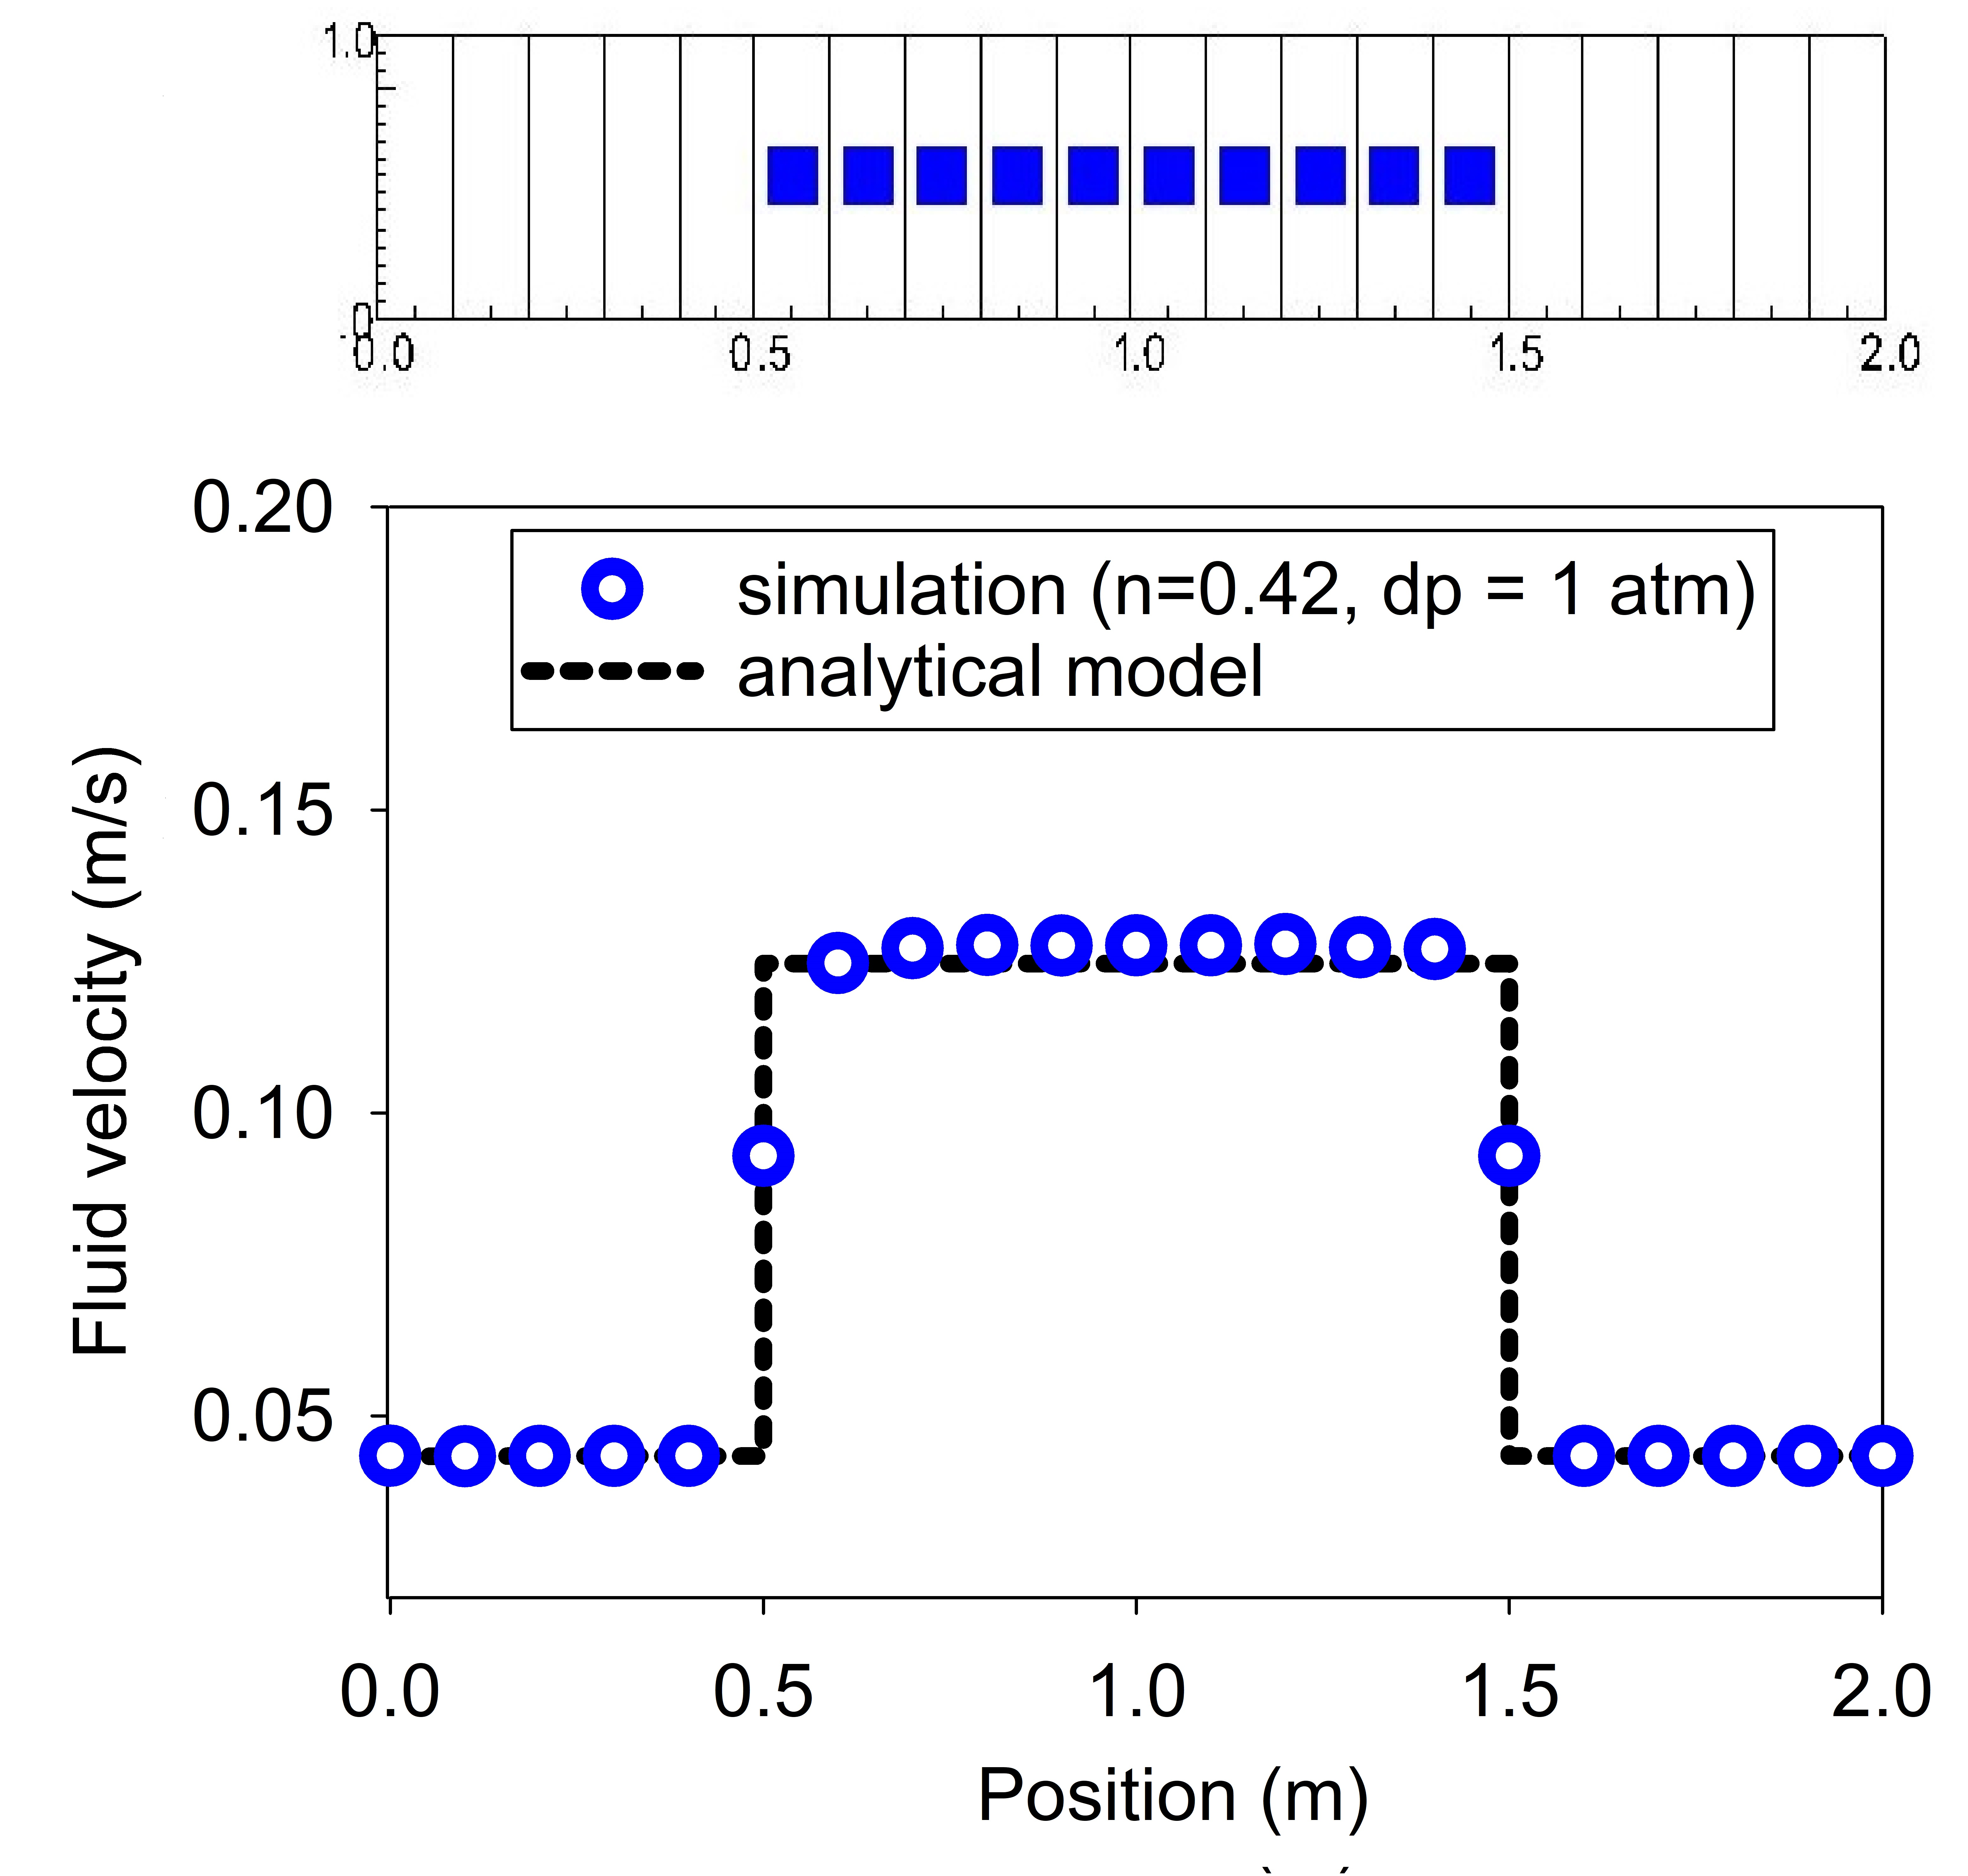
\includegraphics[width=\linewidth]{porousflow1.jpg}
\caption{}
\label{fig:3c}
\end{subfigure}\hfill    
\begin{subfigure}[d]{0.5\linewidth}
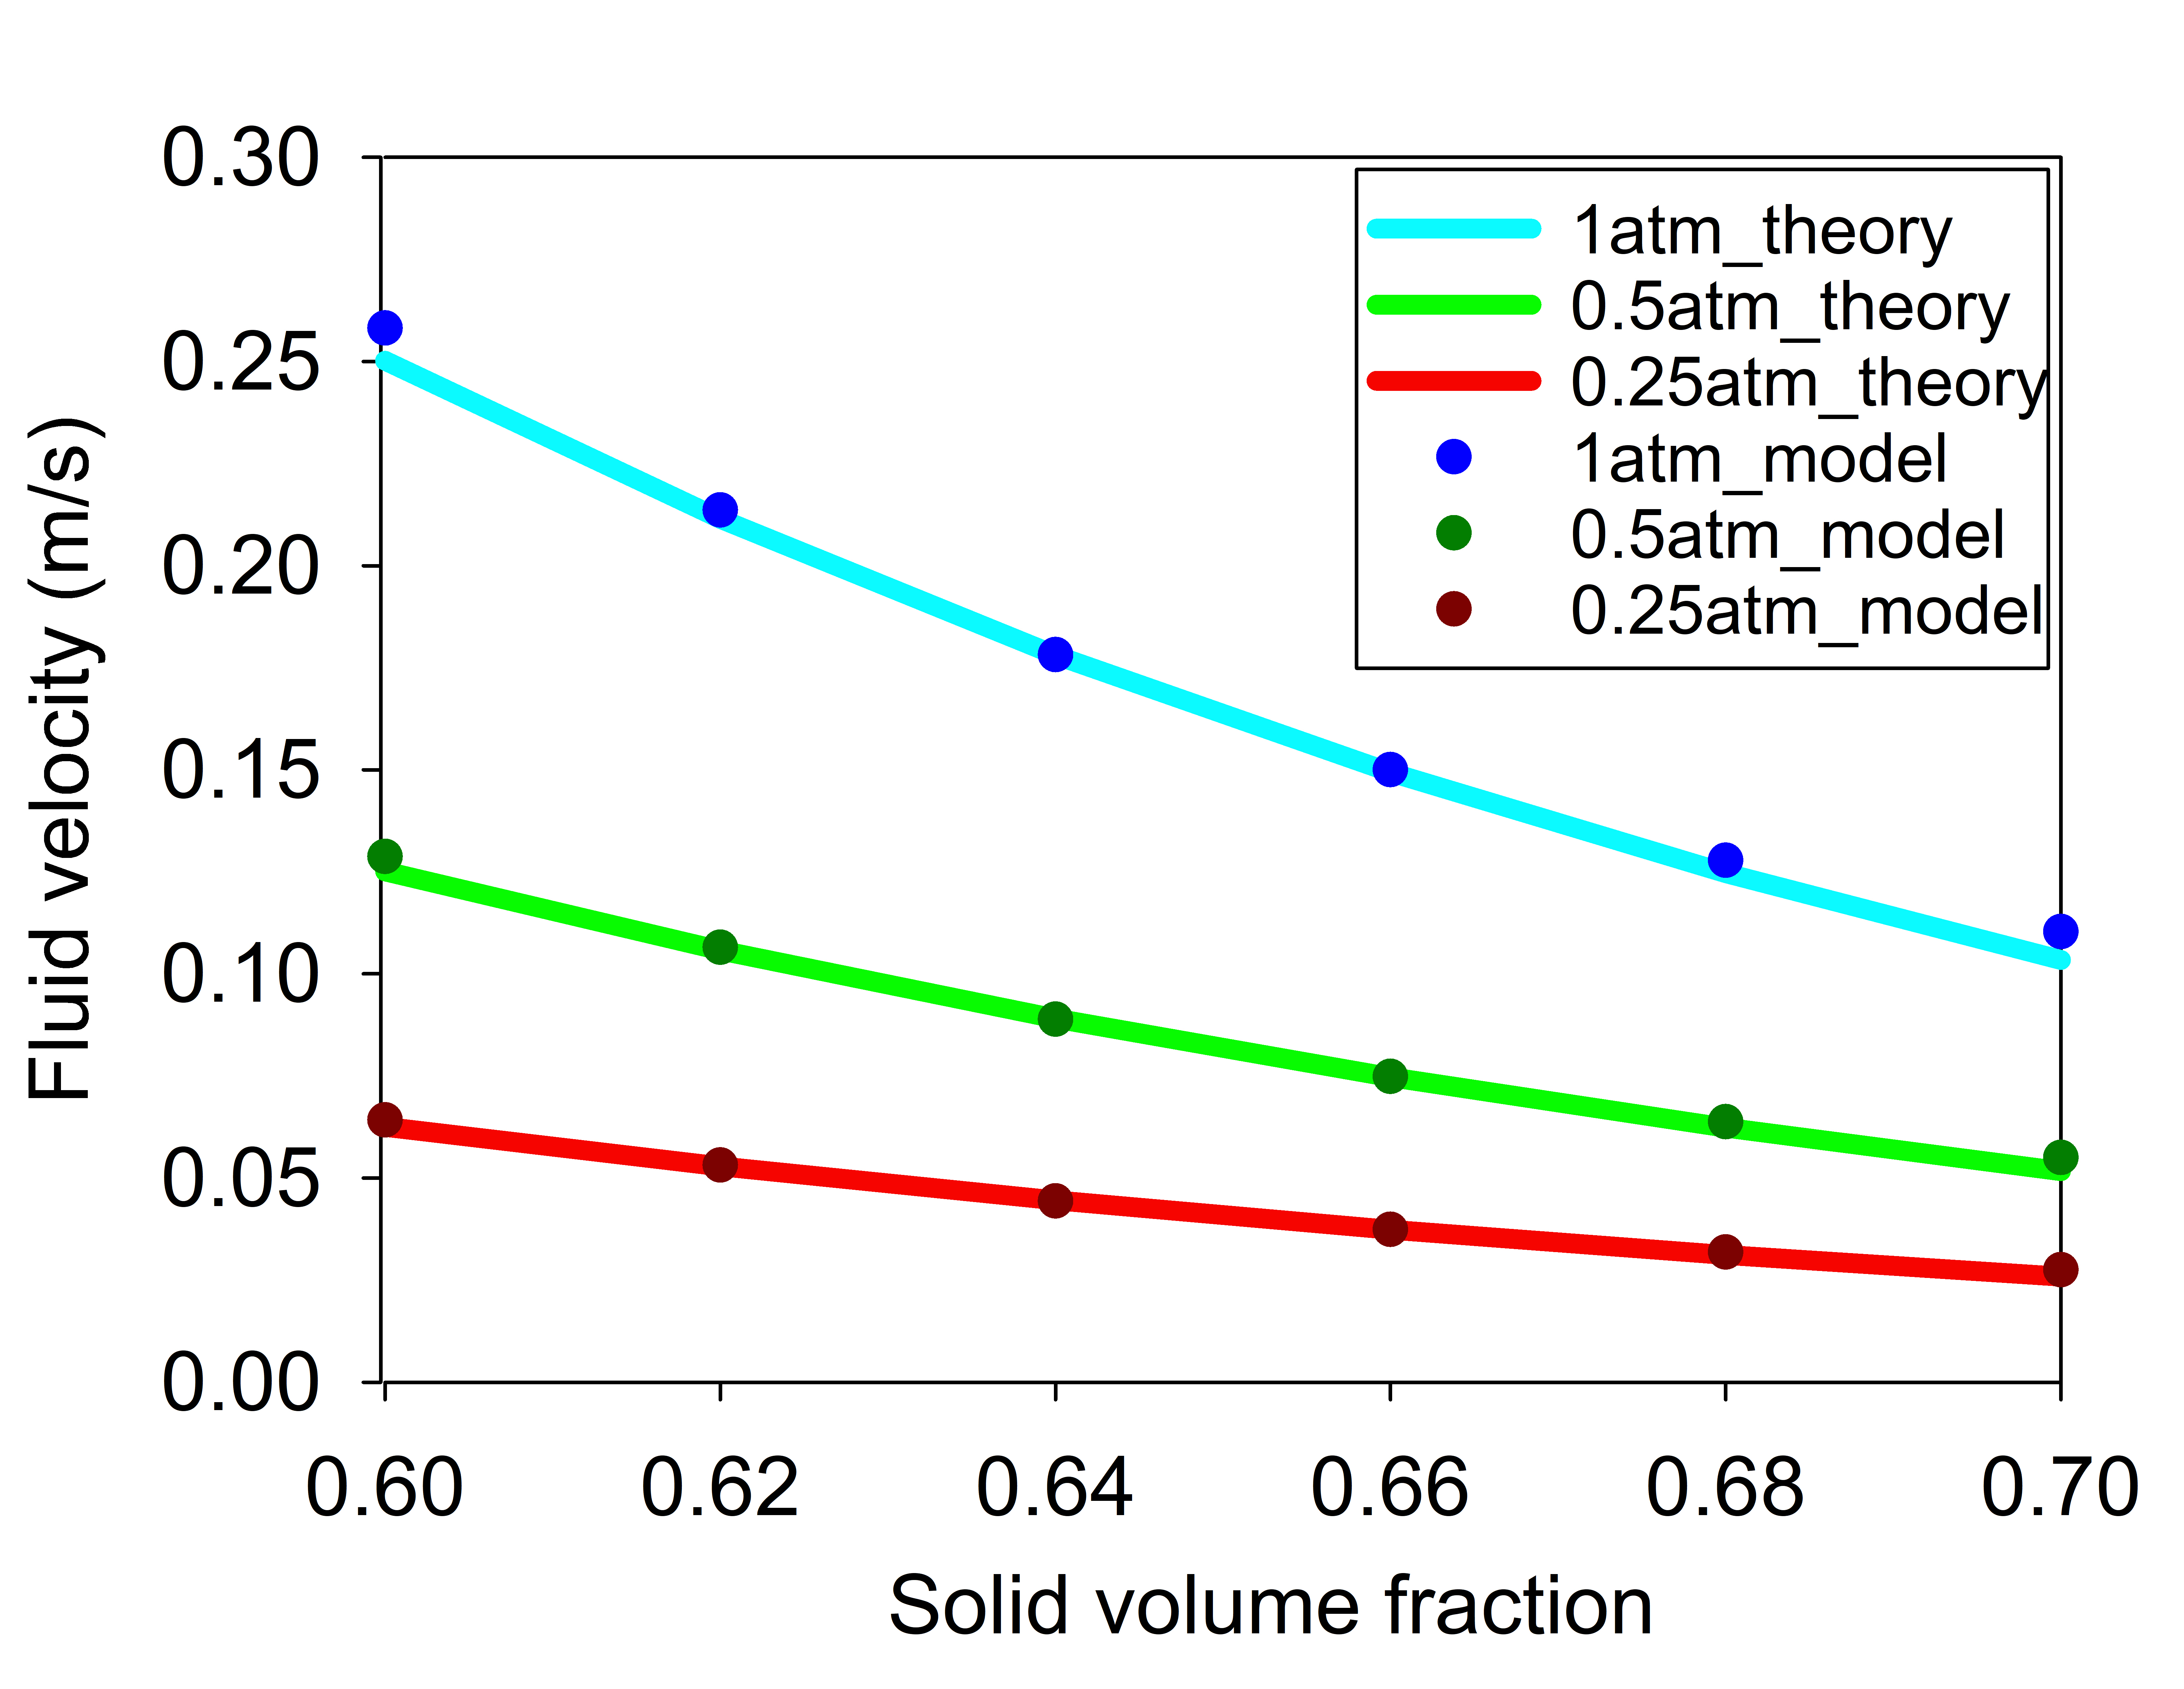
\includegraphics[width=\linewidth]{porousflow.jpg}
\caption{}
\label{fig:3d}
\end{subfigure}
\caption{(a) Discretization of the model and (b) comparision between analytical model and simulation}
\label{fig:porousflow}
\end{figure}
%
%
Our numerical model is validated by modeling fluid flow through a 1m long porous media. This fluid has water properties (bulk modulus is 2GPa, density is 998 kg/m3 at 5 degrees Celsius and 10325 Pa (1atm) pressure, dynamic viscosity $\mu$ is 1mPa s). The porous media is modeled by elastic material with Young's modulus is 10 MPa, Poisson's ratio is 0.3, and density is 2650 kg/m3. The volume fraction of porous media $\phi_s$ is [0.6, 0.62, 0.66, 0.68, 0.7] and the average grain diameter $d$ is 1mm. The model is discretized in 20 finite element and the porous media in 10 finite element with 1 material point per element. The pressure gradient is applied with three different value [0.25, 0.5, 1] atm. Figure \ref{fig:porousflow} shows the comparision of fluid flow prediction between the theory and the model. \\
%
%_______________________________
\subsection{\textsf{Isothermal consolidation}}
A common benchmark fo a fully saturated porous meida is the simulation of one-dimensional consolidation. Using the Carman-Kozeny formula, the time-dependent pressure can be caluated as:
%
%
\begin{equation}
  p_f  = \sum_{m=1}^{\infty} \frac{2F_{ext}}{M} \sin (\frac{Mz}{H}) e^{-M^2T_V} \textrm{    with    }   M = \frac{\pi}{2} (2m+1)
\end{equation}
%
%
where the consolidation rate $T_v =C_vt/H^2$, the consolidation coefficient $C_v = E_v n^3 d^2/(180(1-n)^2\mu) $ and the Oedometer modulus $E_v = E(1-\upsilon)/(1+\upsilon)/(1-2\upsilon)$.

%
%
\begin{figure}
\center
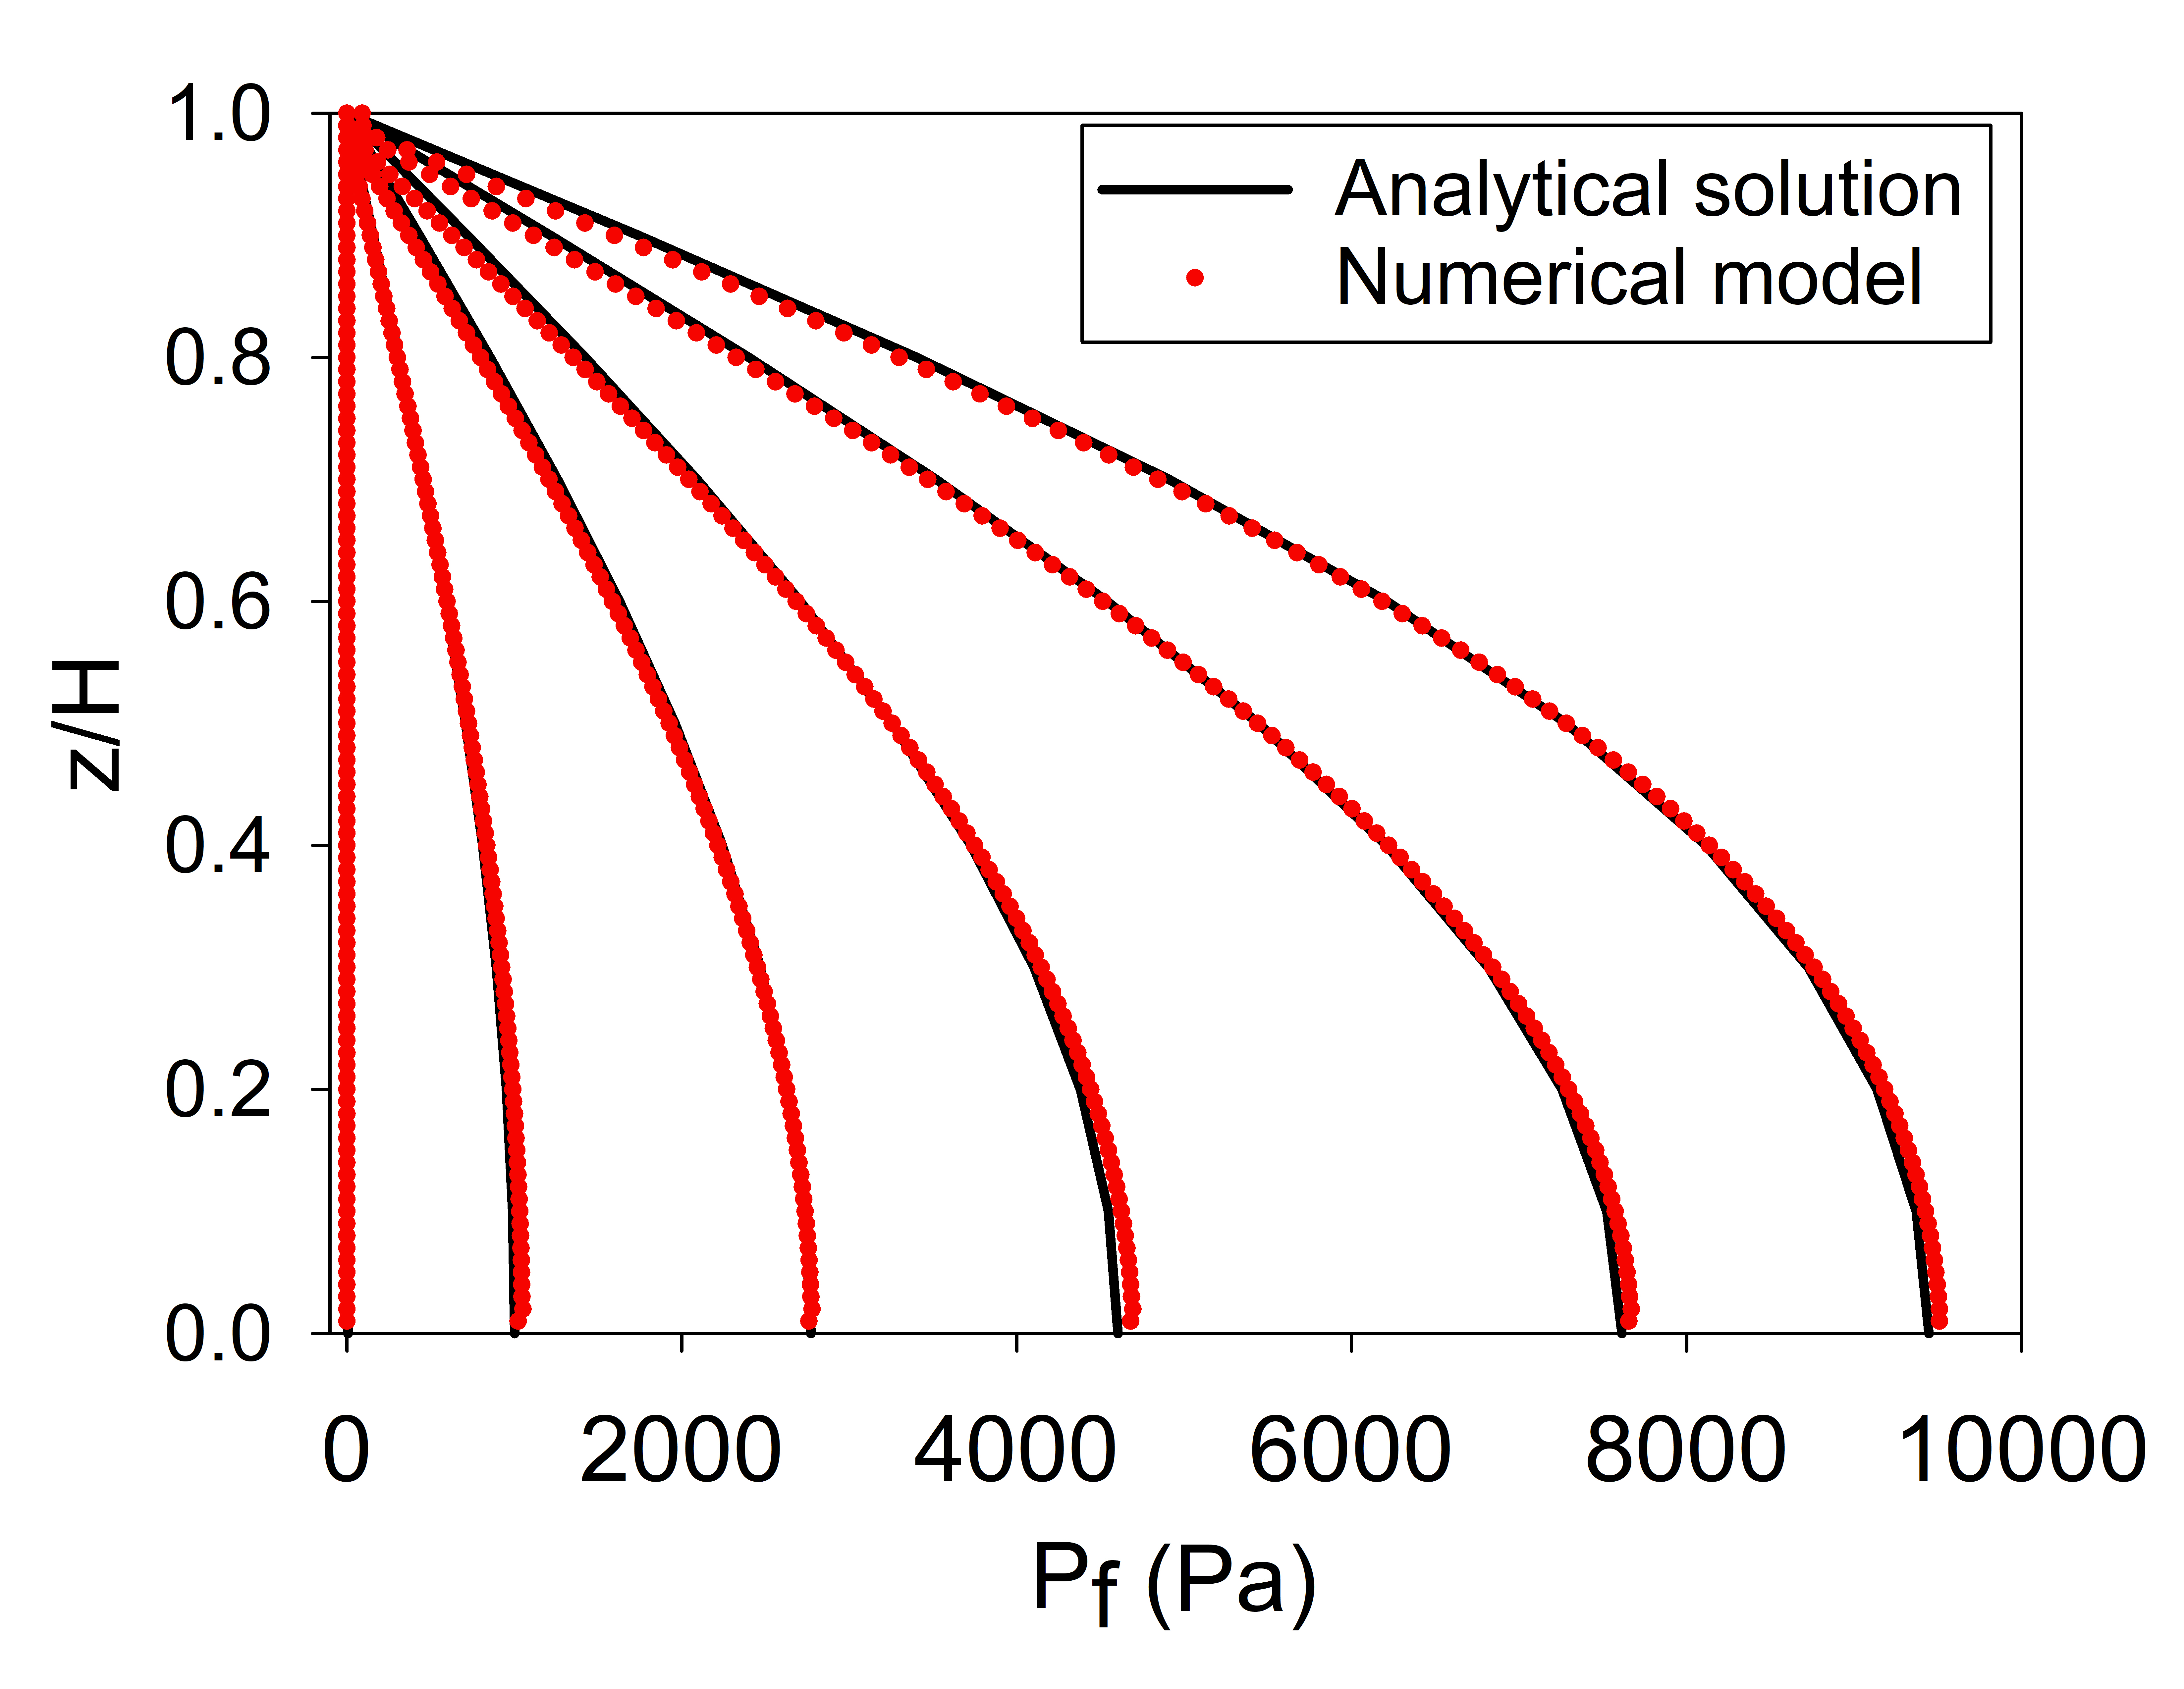
\includegraphics[scale=.3]{consolidation.jpg}
\caption{Compasion between analytical solution and numerical solution}
\label{fig:consolidation}
\end{figure}
%
%
Our numerical model is validated by modeling the consolidation of a 1m column. This fluid has water properties (bulk modulus is 2GPa, density is 998 kg/m3 at 5 degrees Celsius and 10325 Pa (1atm) pressure, dynamic viscosity $\mu$ is 1mPa s). The porous media is modeled by elastic material with Young's modulus is 10 MPa, Poisson's ratio is 0.3, and density is 2650 kg/m3. The volume fraction of porous media $\phi_s$ is 0.7 which is equivalent to the porosity of 0.3 and the average grain diameter $d$ is 1mm. The model is discretized in 100 finite element with 1 material point per element. The external pressure applies to the top of the column is 10 kPa. Figure \ref{fig:consolidation} shows the comparision of fluid flow prediction between the theory and the model. \\

%_______________________________
\subsection{\textsf{thermal induced cavity flow}}
Another benchkmark is the thermal induced cavity flow in porous media. Temperature and velocity distributions are calculated for a square non-deformable saturated porous media The top and bottom walls are insulated, and the left and right walls are at fixed temperatures differing by 1 K. The fluid motion at stead state are cavity flow due to the temperature induced density variation. \\
%
%
\begin{figure}
\center
%add desired spacing between images, e. g. ~, \quad, \qquad, \hfill etc. 
%(or a blank line to force the subfigure onto a new line)
\begin{subfigure}[c]{0.5\linewidth}
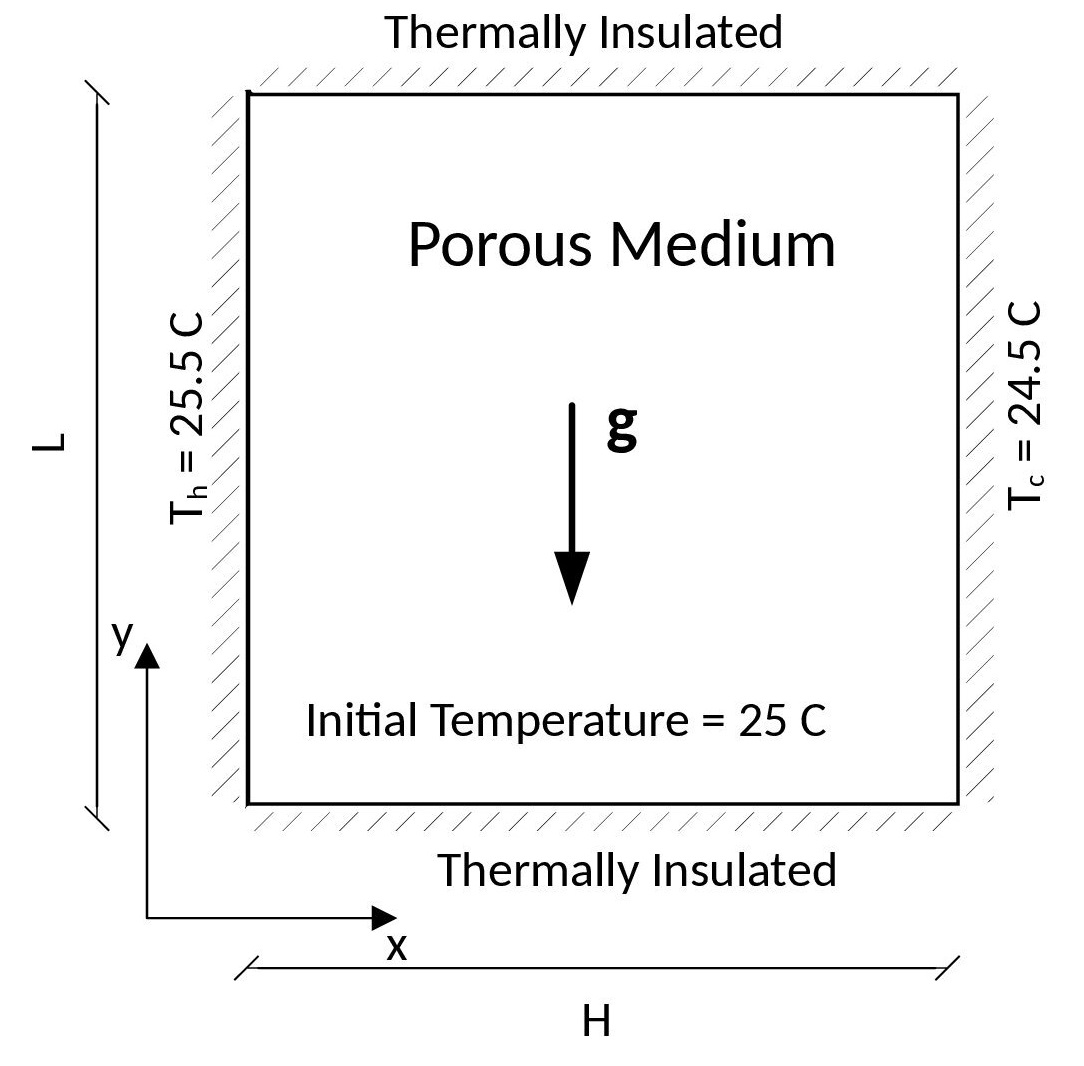
\includegraphics[width=\linewidth]{box_thermal.jpg}
\caption{}
\end{subfigure}\hfill    
\begin{subfigure}[d]{0.5\linewidth}
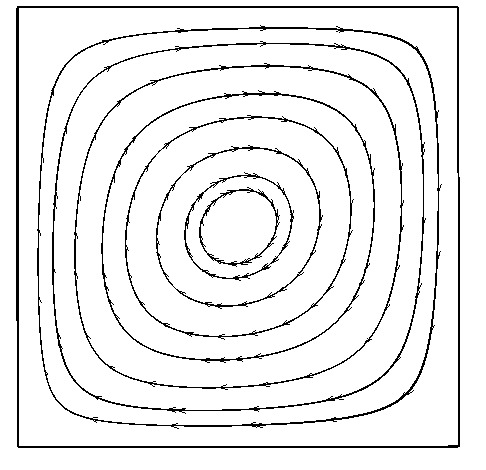
\includegraphics[width=\linewidth]{velocity_thermal-1.jpg}
\caption{}
\end{subfigure}
\caption{(a) Discretization of the model and (b) comparision between analytical model and simulation}
\label{fig:thermal}
\end{figure}
%
%
The numerical is validated by comparing with the numerical solution of the finite element method. The fluid has water properties (bulk modulus is 2GPa, density is 998 kg/m3 at 5 degrees Celsius and 10325 Pa (1atm) pressure, dynamic viscosity $\mu$ is 1.5mPa s). The porous media is modeled by non deformable material, and density is 2500 kg/m3. The specific heat capacity of the water and porous skeleton are 4181 J/kg.K and 835 J/kg.K respectively. The thermal conductivity of the water and porous skeleton are x and x. The volume fraction of porous media $\phi_s$ is 0.6 which is equivalent to the porosity of 0.4 and the average grain diameter $d$ is 1mm. The model is discretized in x finite element with x material point per element. Figure \ref{} shows the numerical results of the model compared with the numerical solution of the finite element method. \\
%_______________________________
\subsection{\textsf{debris flow}}

%_______________________________
\subsection{\textsf{granular column collapse}}

%_______________________________
\subsection{\textsf{earthquake-induced submarine landslides}}

%_______________________________
\section{\textsf{Conclusions}}

%_______________________________
\section{\textsf{Appendix}}

\label{label}

%% The Appendices part is started with the command \appendix;
%% appendix sections are then done as normal sections
%% \appendix

%% \section{}
%% \label{}

%% If you have bibdatabase file and want bibtex to generate the
%% bibitems, please use
%%
%%  \bibliographystyle{elsarticle-num} 
%%  \bibliography{<your bibdatabase>}

%% else use the following coding to input the bibitems directly in the
%% TeX file.

\begin{thebibliography}{00}

%% \bibitem{label}
%% Text of bibliographic item

\bibitem{}

\end{thebibliography}
\end{document}
\endinput
%%
%% End of file `elsarticle-template-num.tex'.
